The primary attack of concern for all blockchain and DLT platforms is the subversion of their consensus protocol and is generally referred as a 51\% attack. Such attack is made possible when an entity or group of entities collude to have enough influence on the network to produce a block or ledger state update with invalid transactions, in the attempt to alter the ledger integrity. Depending on the protocol, the influence can be in computing power or number of nodes and exceeds 50\% of the relevant resource. \\

An attack could be performed for many reasons aside attempting to steal money from a network, including to discredit or shake trust in a network. A consequence of a successful attack would likely be to reduce token prices. Although there is no tangible proof of this, it could explain why 51\% attacks are not too common. Nevertheless, it remains important to prevent and mitigate the risk of an attack as much as possible.\\

The probability of a 51\% attack ($P_{51}$) typically depends on the algorithm used to produce a valid block or ledger update.When considering PoW-based algorithms, $P_{51}$ can be expressed as a function of the hash rate of network nodes. Since the consensus-based protocol on the Catalyst network as laid out in section \ref{Cha:CM} does not rely on solving a cryptographic puzzle, the concept of hash rate of nodes involved in the ledger state update is not relevant to quantify the probability or the cost of an attack on Catalyst network. The number of nodes involved in the production of a ledger state update is however relevant, as explained in this section. \\ 

The probability of a successful 51\% attack on Catalyst network implies that a malicious entity (or group of entities) succeeds in controlling more than half the producer nodes selected to produce the ledger state update during a ledger cycle, giving that entity the power to tamper with the ledger state. The probability $P_{51}$ depends on the following parameters:
\begin{itemize}
\item $N$ : the total number of nodes in the worker pool. 
\item $P$ : the subset of worker nodes selected to perform work for one ledger cycle ($P \leq N$).
\item $O$ : the number of malicious nodes in the worker pool ($0 \leq O \leq N$). This is a total subset of malicious nodes colluding to perform an attack on the network.
\item $p$ : the number of malicious nodes in the subset $P$ of producers. ($0 \leq p \leq P$).
\end{itemize}
An attack can be considered successful for any value $p \in [p_0,P]$ where $p_0 = P/2 + 1$ which is equivalent to $p > 50\%P$. When $P \approx N$, \textit{i.e.} the number of producers selected during a ledger cycle is very close to the total number of nodes in the worker pool, the absence of a randomness element in the selection of $P$ producers makes it easy to compute the probability of a successful attack on the network: $P_{51} \approx O/N$. A malicious entity would know exactly when an attack can successfully be performed, that is when $O > N/2$. \\

When $N \gg P$, $P_{51}$ can there be expressed by the discrete sum:
\begin{equation}
\label{eq:1}
P_{51} = \sum_{p=p_0}^{P} P_{A}(p)
\end{equation}
where $P_{A}(p)$ represents the probability of having $p$ malicious nodes in the set $P$. When the ratio between the total number of nodes $N$ and the number of nodes $P$ is large ($N > 20\times P$) it can be expressed as follows: 
\begin{equation}
\label{eq:2}
P_{A}(p) = \frac{\overbrace{\left( \begin{array}{c} O \\
p \end{array} \right)}^\text{A} 
\overbrace{\left( \begin{array}{c} N - O \\ P - p \end{array} \right)}^\text{B}}{\underbrace{\left( \begin{array}{c} N \\
P \end{array} \right)}_\text{C}}
\end{equation}
$A$ represents the number of possible combinations for choosing $p$ nodes from $O$ malicious nodes. $B$ represents the number of possible combinations for choosing good (non-malicious) nodes for the remaining $N-O$ nodes in the worker pool. Finally, $C$ corresponds to the number of available combinations for choosing $P$ nodes from the pool of $N$ nodes.\\
\\
In equation \ref{eq:2}, $P_A(p)$ is the probability mass function of a hypergeometric distribution over the set of parameters $\{N,O,P\}$. Note that such expression is valid for $max(0,O+P-N) \leq p \leq min(O,P)$. \\

There are two main arguments behind having a large number of $N$ nodes:

\begin{itemize}
 \item To account for the fact that most nodes with sufficient resources may want to join the worker pool and receive tokens as reward for their contribution to the ledger state management
\item To make it increasingly costly for any malicious entity to control more than half the nodes.
\end{itemize}

\begin{comment}
As explained in section~\ref{Sec:Reg}, prior to joining the worker pool, nodes are part of a work queue. Nodes in the worker pool are granted a work pass valid for finite period time. When a node $W_j$ joins the worker pool, it is granted a work pass defined by a decay rate $\lambda_j$. Similarly to unstable nuclear elements the work pass has a 50\% chance to remain valid after $W_j$ sits in the worker pool for a period of time $ln(2)/\lambda_j$. The decay rate is not fixed over time but instead can very depending on the quality of work produced by $W_j$ when selected to be a producer. The quality of work performed by a producer during a ledger cycle $\mathcal{C}_n$ can be estimated by verifying if the producer identifier is found in the lists $\mathcal{L}_n(prod)$ and $\mathcal{L}_n(vote)$. If the identifier is found in one of the two lists or none, the decay rate increases. $\lambda_j$ can also vary to account for the demand of work, \textit{i.e.} the length of the work queue, although a threshold is considered to mitigate the risk of a malicious entity (or group of entities) trying to simulate a highest demand for work than reality.
\end{comment}
As explained in section~\ref{Sec:Reg}, prior to joining the worker pool, nodes are part of a work queue. Nodes in the worker pool are granted a work pass valid for finite period time. As a result, a varying number of nodes leaves the worker pool at each ledger cycle. Although the size of the worker pool might be constant ($N$ nodes), the selection of nodes actually forming the worker pool changes over time. The mechanism used to define a score for nodes in the work queue is designed to prevent malicious nodes from gaining control of a large fraction of worker nodes. Nevertheless, as we derive the probability $P_{51}$ in this section, we must stress that the fraction $O/N$ may change (increase or decrease) over time and should be taken into account if computing the probability over a series of ledger cycles.\\

When $N \gg P$ the probability of a successful attack can therefore be estimated using the cumulative hypergeometric distribution function (CDF) for $p \in [p_0,P]$. In this paper, we provide probability estimate obtained using $scipy.stats$ Python library. The graphs presented are obtained using $matplotlib.pyplot$ library. Rather than computing the CDF, the probability measurements are obtained using the survival probability (SDF), which is the inverse of CDF but is known to provide more accurate results\footnote{See https://docs.scipy.org/doc/scipy-0.14.0/reference/generated/scipy.stats.hypergeom.html for more details.}. \\

As an example, assume a rather large number of nodes in the worker pool, $N = 20,000$, out of which $5\%$ are selected as producers for a given cycle ($P = 1,000$). \\

Further assume a ratio $O/N=20\%$, \textit{e.g.} $1$ every $5$ nodes in the worker pool is controlled by a malicious entity ($O=4000$). The probability of a successful attack is calculated using the SDF of an hypergeometric distribution using these set of parameters and amounts to: $P_{51} = 1-SDF(20000,4000,1000) \approx 10^{-9}\%$. For the same set $(N,P)$, the probability of a successful attack reaches $0.04\%$ for $O/N=45\%$ of malicious nodes in the worker pool. \\

Figure \ref{fig:P} shows the probability of a successful control of more than 50\% of the producers as a function of the number of producers for four different worker pool sizes and two attack scenarios: when a malicious entity controls $O/N = 45\%$ of the worker nodes in blue, and in orange when a malicious controls $O/N = 35\%$ of the worker nodes in blue. For $N=20000$, the probability remains below $10^{-9}$ if $P < \approx 4000$ while for a smaller worker pool size ($N=5000$), the ratio $P/N$ must be at close to 50\% to prevent a successful control of more than 50\% of the producers. 

\newpage

\begin{figure}[H]
\centering

 \begin{subfigure}[b]{0.45\textwidth}
        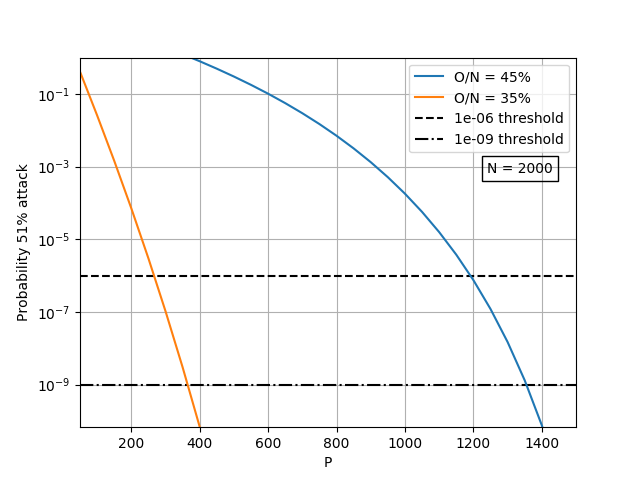
\includegraphics[width=\textwidth]{Figures/Prob51_vs_P_N2000_O35_to_45}
        \renewcommand{\thesubfigure}{a}
     \caption{$N = 2000$}
        \label{fig:N2000}
    \end{subfigure}
    \begin{subfigure}[b]{0.45\textwidth}
        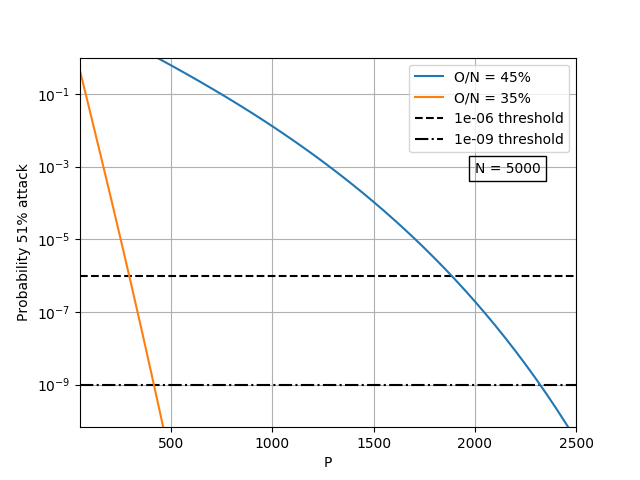
\includegraphics[width=\textwidth]{Figures/Prob51_vs_P_N5000_O35_to_45} 
        \renewcommand{\thesubfigure}{b}
        \caption{$N = 5000$}
        \label{fig:N5000}
    \end{subfigure}
        \begin{subfigure}[b]{0.45\textwidth}
        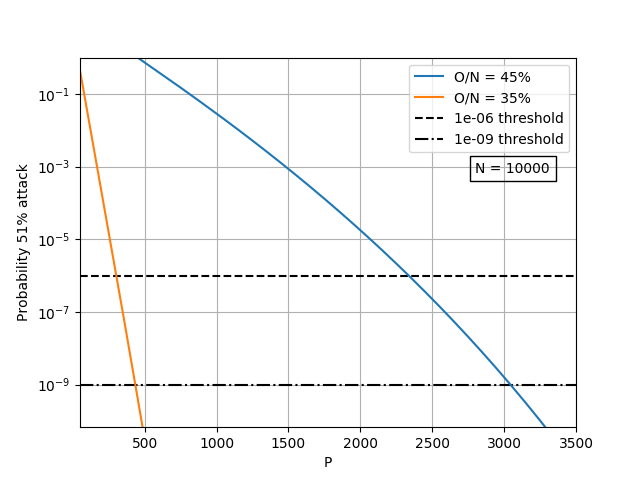
\includegraphics[width=\textwidth]{Figures/Prob51_vs_P_N10000_O35_to_45}  
       \renewcommand{\thesubfigure}{c}
        \caption{$N = 10000$}
        \label{fig:N10000}
    \end{subfigure}
        \begin{subfigure}[b]{0.45\textwidth}
        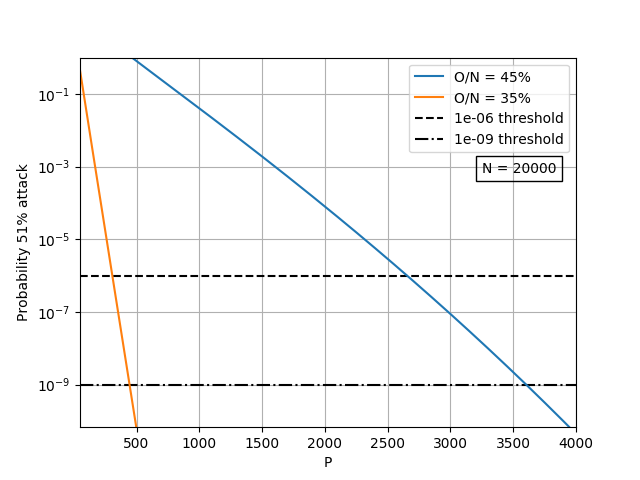
\includegraphics[width=\textwidth]{Figures/Prob51_vs_P_N20000_O35_to_45}
        \renewcommand{\thesubfigure}{d}
        \caption{$N = 20000$}
        \label{fig:N=20000}
    \end{subfigure}
\caption{Probability of 51\% attack as a function of P for various worker pool size ($N=\{2000, 5000, 10000, 20000\}$) when a malicious entity controls $O/N = 45\%$ of the worker nodes in blue, and in orange when a malicious controls $O/N = 35\%$}\label{fig:P}
\end{figure}    

Figure \ref{fig:threshV} displays the minimum ratio $P/N$ required to maintain a probability below $10^{-6}$ and $10^{-9}$ for various malicious scenario ($O/N$ ratio between 30\% and 45\%) . This shows that as $N$ increases the required $P/N$ ratio required for the same security level decreases. 

\begin{figure}[H]
	\centering
	\begin{subfigure}[b]{0.45\textwidth}
		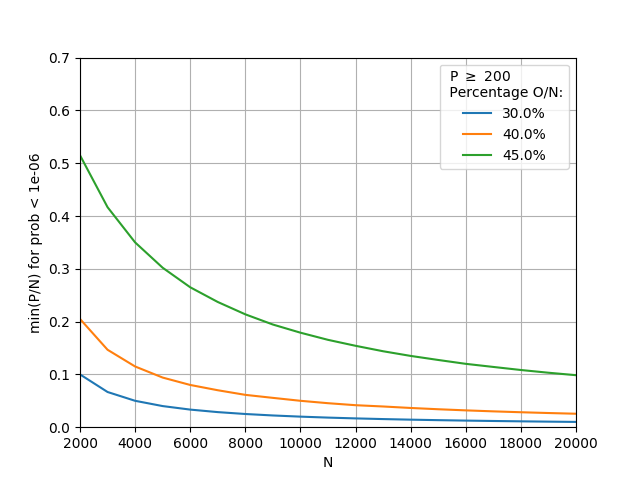
\includegraphics[width=\textwidth]{Figures/PoN_vs_N_Thre_Prob51_10em6_O30_to_45}
		
		\renewcommand{\thesubfigure}{a}
		\caption{Prob. Attack = $10^{-6}$}
		\label{fig:N20-50}
	\end{subfigure}
	\begin{subfigure}[b]{0.45\textwidth}
		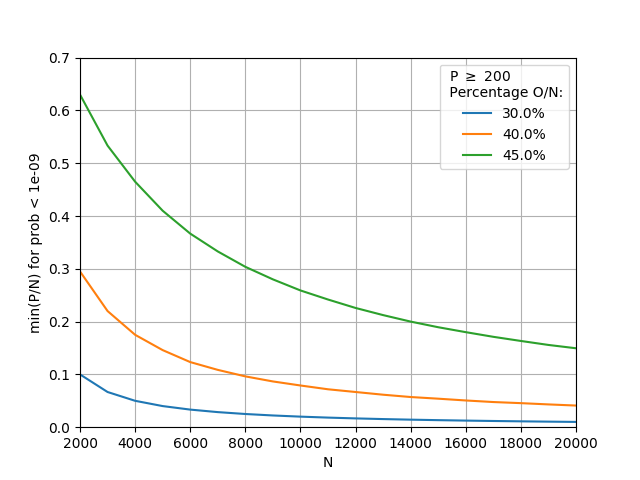
\includegraphics[width=\textwidth]{Figures/PoN_vs_N_Thre_Prob51_10em9_O30_to_45}
		
		\renewcommand{\thesubfigure}{b}
		\caption{Prob. Attack = $10^{-9}$}
		\label{fig:N50-100}
	\end{subfigure}
\caption{\label{fig:threshV} This graph shows the $P/N$ ratio required for a probability of a 51\% attack of less than $10^{-6}$ on a validation cycle versus $N$. This is shown against various $O/N$ ratio. }
\end{figure}

This series of graphs gives a good indication on what pair of parameters ($N,P$) to consider for a high resilience to 51\% attack. Given a number of nodes in the worker pool, we can deduce the number of producer nodes to select during one ledger cycle. Inversely, given a selected number of producers for a ledger cycle, we can define a minimum size for the worker pool. As detailed in the next section, the number of producers selected for a ledger cycle is important to ensure that a consensus can be reached on the correct ledger state update to distribute to the rest of the network.

%In section~\ref{subsec:comp}, we consider the fact that a producer may not collect exactly $P$ local hashes during the first ledger cycle phase. We argue that a threshold $P_{min}$ should apply to decide whether a majority of producers build the same local hash. 
